\documentclass[10pt,twocolumn]{article}
\usepackage[margin=0.72in]{geometry}
\usepackage{amsmath,amssymb,amsthm}
\usepackage{booktabs}
\usepackage{graphicx}
\usepackage{xcolor}
\usepackage{xurl}
\usepackage{hyperref}
\usepackage{microtype}

\hypersetup{
  colorlinks=true,
  linkcolor=blue!60!black,
  citecolor=blue!60!black,
  urlcolor=blue!60!black
}

\title{\textbf{Formal Algebraic and $\mathbb{F}_2$-Circuit Certification for the NP-Completeness of Optimal CNOT Synthesis on Linear Oracles}}
\author{Lluis Eriksson\\
\small Independent Researcher \quad $\cdot$ \quad \texttt{CNOT-HARD-CERT-1.0}\\
\small \url{https://github.com/lluiseriksson/optimal-cnot-hardness-certificates}}
\date{November 26, 2026}

\begin{document}
\maketitle

\begin{abstract}
We present a machine-checked constructive Lean~4.35.0 kernel and zero-float $\mathbb{F}_2$ circuit verification suite (\texttt{CNOT-HARD-CERT-1.0}) auditing Andreas Pavlogiannis's proof that optimal CNOT synthesis is NP-complete even for involutive linear oracles $B_G \in \mathrm{GL}(n+1+m, 2)$ and even with free SWAP gates or ancillas (\texttt{arXiv:2611.34138v1}, Nov.\ 2026). Our artifact combines 18 constructive Lean~4.35.0 theorems (\texttt{0 sorry}, \texttt{0} custom axioms, \texttt{0 Classical.choice}, \texttt{0} warnings), an AST-audited zero-float Python $\mathbb{F}_2$ bitmask verifier, 16 canonical JSON certificates (\texttt{C01}--\texttt{C16}), and 36 unit and forgery-rejection tests. In Lean we formalize linear-oracle involution, 3-CNOT SWAP equivalence, free-ancilla reduction rules, Lemma~2 clique-cover dominance and evenness, Lemma~3 gate-elimination Case~(a)/(b) projections and telescoping step, Lemma~4 Hamiltonian-path CNOT wire invariants, $z$-wire restoration, and exact gate count $2m + \tau(G) + 1$, and Theorem~5 parity-rounding reduction soundness. In Python we execute the Lemma~2 reduction $H \mapsto H_1 \cup H_2 \cup K_{2n}$ with exact branch-and-bound vertex covers, step-by-step Lemma~3 gate elimination on optimal and Case-(b) XOR circuits, full $\mathbb{F}_2$ matrix simulation of synthesized Lemma~4 CNOT circuits up to $\mathrm{GL}(33,2)$ with $B_G^2 = I$, and syntactic free-SWAP/clean-ancilla to XOR translation.
\end{abstract}

\section{Introduction and Audited Scope}

Given an invertible binary matrix $A \in \mathrm{GL}(d, 2)$ and a gate budget $K \in \mathbb{N}$, the \emph{optimal CNOT synthesis} problem asks whether $A$ can be implemented using at most $K$ in-place CNOT gates $x_j \leftarrow x_j \oplus x_k$. Building on the XOR-circuit edge-form lower bound of Boyar, Matthews, and Peralta~\cite{boyar2013} ($D_{\mathrm{XOR}}(F_G) = m + \tau(G)$ for $F_G = \{z \oplus x_u \oplus x_v\}_{\{u,v\} \in E}$, where $\tau(G)$ is the minimum vertex cover size of $G = (V, E)$ with $|V|=n, |E|=m$), Pavlogiannis~\cite{pavlogiannis2026cnot} proves NP-completeness directly on \emph{linear oracles}
\begin{equation}
  B_G = \begin{pmatrix} I_{n+1} & 0 \\ F_G & I_m \end{pmatrix} \in \mathrm{GL}(n+1+m, 2), \qquad B_G^2 = I,
\end{equation}
via four modular pillars: (i)~Lemma~2 reduces general Vertex Cover on $H$ to $G = H_1 \cup H_2 \cup K_{2n}$ with $\tau(G) = 2\tau(H) + 2n$ even and a minimum vertex cover inducing a Hamiltonian path; (ii)~Lemma~3 proves $D_{\mathrm{XOR}}(F_G) = m + \tau(G)$ by localized gate elimination; (iii)~Lemma~4 proves $D_{\mathrm{XOR}}(B_G) = 2m + \tau(G)$ and $D_{\mathrm{CNOT}}(B_G) \in \{2m+\tau(G), 2m+\tau(G)+1\}$ via an explicit Hamiltonian-path CNOT synthesis; and (iv)~Theorem~5 reduces $\tau(G) \le k$ to $D_{\mathrm{CNOT}}(B_G) \le 2m + k' + 1$ ($k'$ rounded down to even), persisting under free SWAPs and free ancillas.

This note provides an independent machine-checked audit (\texttt{CNOT-HARD-CERT-1.0}) with an explicit scope split:
\begin{enumerate}
  \item \textbf{Constructive Lean~4.35.0 kernel} (\path{lean/CnotHardnessCert.lean}): 18 universally quantified Boolean/$\mathbb{F}_2$ and $\mathbb{N}$-arithmetic theorems (\texttt{0 sorry}, \texttt{0 Classical.choice}, audited via \texttt{\#print axioms}) formalizing all algebraic, wire-update, gate-count, telescoping, and parity-reduction steps.
  \item \textbf{AST-audited zero-float $\mathbb{F}_2$ verifier} (\path{src/cnot_hardness_verifier.py}): executes the finite-graph constructions, gate-elimination sequences, full $\mathbb{F}_2$ CNOT matrix simulations, and free-resource syntactic translations across 16 certificates.
\end{enumerate}

\section{Constructive Lean 4.35.0 Kernel}

All 18 theorems in \texttt{CnotHardnessCert.lean} build in $0.93\text{ s}$ under Lean~4.35.0 with zero warnings and depend exclusively on at most \texttt{propext} and \texttt{Quot.sound} (zero \texttt{Classical.choice}, with 9 theorems depending on zero axioms). Table~\ref{tab:lean} summarizes all 18 quantified Lean statements in abbreviated mathematical syntax. Note honestly that Lean certifies the Boolean wire/gate identities, telescoping step, exact gate counts, and Theorem~5 parity-rounding soundness, while finite-graph vertex-cover branch-and-bound, explicit circuit execution, and gate-elimination replays are certified by our zero-float $\mathbb{F}_2$ Python verifier in Section~\ref{sec:modes}.

\begin{table*}[t]
\centering
\caption{Summary of all 18 constructive theorems in \texttt{CnotHardnessCert.lean} (Lean~4.35.0, \texttt{0 sorry}, \texttt{0 Classical.choice}, \texttt{0} warnings).}
\label{tab:lean}
\scriptsize
\setlength{\tabcolsep}{3pt}
\begin{tabular}{@{}rll@{}}
\toprule
\# & Lean Theorem Name & Quantified Lean Statement (abbreviated mathematical syntax) \\
\midrule
1 & \texttt{linear\_oracle\_involution} & $\forall y, f \in \mathbb{B},\; (y \oplus f) \oplus f = y$ (0 axioms) \\
2 & \texttt{reversible\_edge\_form\_involution} & $\forall y,z,x_u,x_v \in \mathbb{B},\; (y \oplus (z \oplus (x_u \oplus x_v))) \oplus (z \oplus (x_u \oplus x_v)) = y$ (0 axioms) \\
3 & \texttt{three\_cnot\_swap\_exact} & $\forall a,b \in \mathbb{B},\; a_1=a\oplus b,\, b_1=b\oplus a_1,\, a_2=a_1\oplus b_1 \implies (a_2,b_1)=(b,a)$ (0 axioms) \\
4 & \texttt{ancilla\_zero\_control\_and\_target} & $\forall c,t \in \mathbb{B},\; (t \oplus \bot = t) \land (\bot \oplus c = c)$ (0 axioms) \\
5 & \texttt{lemma2\_clique\_cover\_dominance} & $\forall n \ge 1,\, \tau_H \le n-1,\; 2\tau_H + 2n < 4n - 1$ \\
6 & \texttt{lemma2\_even\_and\_threshold\_iff} & $\forall n,\tau_H,k,\; (2\tau_H+2n)\bmod 2 = 0 \land (\tau_H \le k \iff 2\tau_H+2n \le 2k+2n)$ \\
7 & \texttt{lemma2\_hamiltonian\_interleaving} & $\forall n \ge 1,\, \tau_H \le n-1,\; 2\tau_H < 2n \land 2\tau_H + (2n-2\tau_H) + 2\tau_H = 2\tau_H + 2n$ \\
8 & \texttt{gate\_elim\_case\_a\_projection} & $\forall z, x_v \in \mathbb{B},\; (z \oplus z = \bot) \land (z \oplus (z \oplus x_v) = x_v)$ (0 axioms) \\
9 & \texttt{gate\_elim\_case\_b\_projection} & $\forall z,x_u,x_w,x_v,\; x_u{=}x_w \to x_u{\oplus}x_w{=}\bot \land z{\oplus}(x_u{\oplus}x_w){=}z \land z{\oplus}(x_u{\oplus}x_v){=}z{\oplus}(x_w{\oplus}x_v)$ (0 ax.) \\
10 & \texttt{gate\_elim\_telescoping\_step} & $\forall c_1\le c_0, e_1\le e_0, t_1\le t_0,\; (e_0-e_1)+(t_0-t_1)\le c_0-c_1 \land e_1+t_1\le c_1 \to e_0+t_0\le c_0$ \\
11 & \texttt{lemma4\_xor\_lower\_bound\_lift} & $\forall c,c',m,\tau,\; c'+m \le c \land m+\tau \le c' \to 2m+\tau \le c$ \\
12 & \texttt{lemma4\_cnot\_wire\_invariant} & $\forall z,y,x_{s_i},x_{s_{i+1}},x_u,\; y_{2a}{=}y{\oplus}z{\oplus}x_{s_i}{\oplus}x_u \land y_{2b}{=}y{\oplus}z{\oplus}x_{s_i}{\oplus}x_{s_{i+1}} \land z_2{=}z{\oplus}x_{s_{i+1}}$ (0 ax.) \\
13 & \texttt{lemma4\_z\_wire\_restored} & $\forall z, x_{s_k} \in \mathbb{B},\; (z \oplus x_{s_k}) \oplus x_{s_k} = z$ (0 axioms) \\
14 & \texttt{lemma4\_cnot\_gate\_count\_exact} & $\forall k \ge 1,\, k-1 \le m,\; 2 + 3(k-1) + 2(m-(k-1)) = 2m + k + 1$ \\
15 & \texttt{theorem5\_even\_budget\_rounding} & $\forall \tau,k,\; \tau\bmod 2=0 \to k'\bmod 2=0 \land (\tau\le k \iff \tau\le k')$ \\
16 & \texttt{theorem5\_reduction\_iff} & $\forall m,\tau,k,d_{\mathrm{cnot}},\; \tau\bmod 2=0 \land 2m+\tau \le d_{\mathrm{cnot}} \le 2m+\tau+1 \to (\tau \le k \iff d_{\mathrm{cnot}} \le 2m + k' + 1)$ \\
17 & \texttt{free\_resource\_sandwich} & $\forall m,\tau,d_{\mathrm{free}},d_{\mathrm{cnot}},\; 2m+\tau \le d_{\mathrm{free}} \le d_{\mathrm{cnot}} \le 2m+\tau+1 \to d_{\mathrm{free}} \in \{2m+\tau, 2m+\tau+1\}$ \\
18 & \texttt{xor\_transitive\_cancellation} & $\forall a, b, c \in \mathbb{B},\; (a \oplus b) \oplus (b \oplus c) = a \oplus c$ (0 axioms) \\
\bottomrule
\end{tabular}
\end{table*}

\section{Zero-Float \texorpdfstring{$\mathbb{F}_2$}{F2} Verification Modes}
\label{sec:modes}

The verifier \path{src/cnot_hardness_verifier.py} is statically AST-audited by \texttt{pytest} for zero floating-point operations, representing every $\mathbb{F}_2$ linear expression and matrix row as an exact Python \texttt{int} bitmask.

\paragraph{Mode 1 (\texttt{promise\_vc\_reduction\_lemma2}, \texttt{C01}--\texttt{C04}).}
Given a source graph $H$ ($n$ vertices), computes exact $\tau(H)$ via branch-and-bound, builds $G = H_1 \cup H_2 \cup K_{2n}$ (with complete bipartite edges between $K_{2n}$ and $H_1 \cup H_2$), verifies $\tau(G) = 2\tau(H)+2n$ independently by exact branch-and-bound on $G$ (up to $n_G = 16$, \texttt{C03}--\texttt{C04}), and checks that the alternating sequence $s_1, u_1, \dots, s_t, u_t, u_{t+1}, \dots, u_{2n}$ is a valid vertex cover inducing a Hamiltonian path in $G[S]$ (Fig.~\ref{fig:l2}).

\begin{figure}[t]
  \centering
  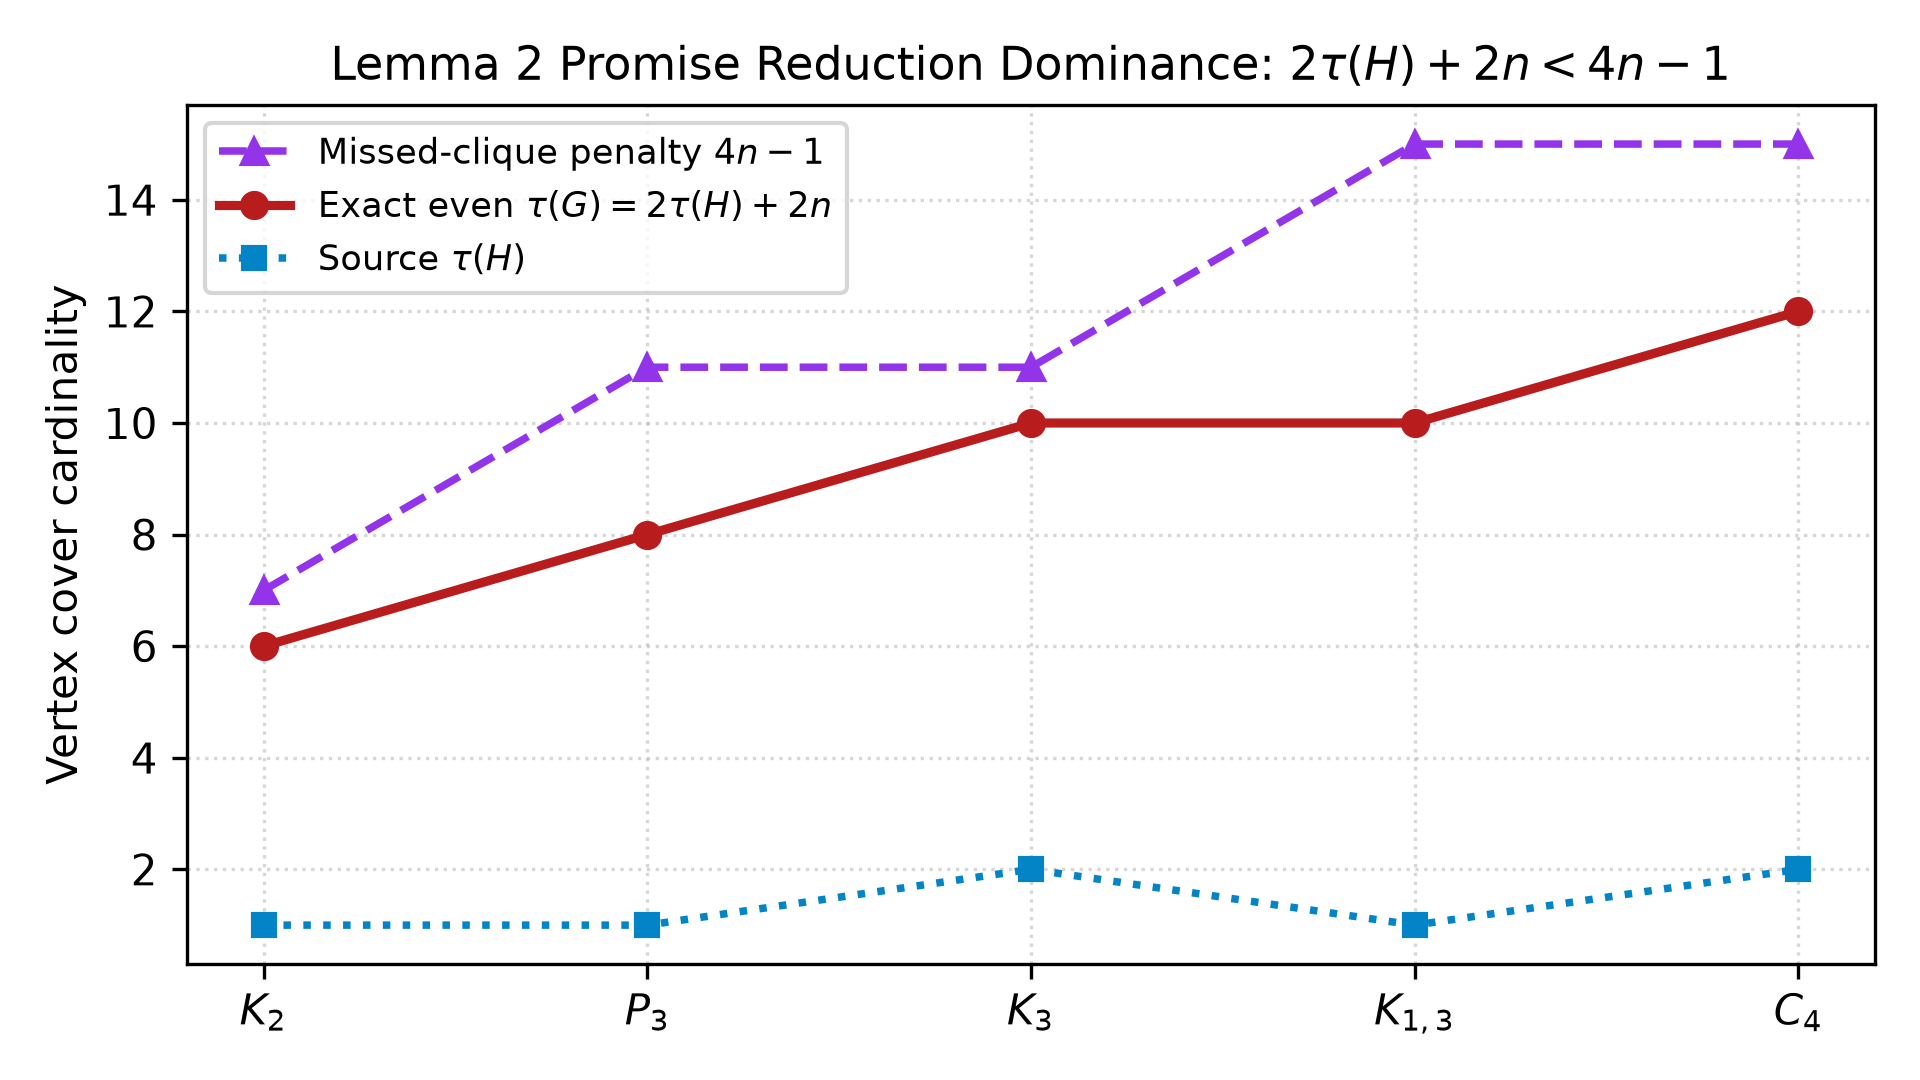
\includegraphics[width=\linewidth]{figures/fig2_lemma2_promise_reduction.png}
  \caption{Lemma~2 promise vertex-cover reduction on $H \in \{K_2, P_3, K_3, K_{1,3}, C_4\}$ confirming strict clique-cover dominance $2\tau(H) + 2n < 4n - 1$.}
  \label{fig:l2}
\end{figure}

\paragraph{Mode 2 (\texttt{gate\_elimination\_lemma3}, \texttt{C05}--\texttt{C08}).}
Given $G$ and a supplied XOR circuit $C$ over $\{z, x_0, \dots, x_{n-1}\}$, verifies that $C$ computes every edge form $z \oplus x_u \oplus x_v$, then \emph{executes} Pavlogiannis's localized gate-elimination sequence $\langle C_0, G_0 \rangle \to \dots \to \langle C_q, G_q \rangle$: locating the first two-input gate $g \leftarrow a \oplus b$, projecting $x_u \mapsto z$ (Case~a, deleting $u$) or $x_u \mapsto x_w$ (Case~b, merging $u$ into $w$), removing all redundant gates, and verifying both invariant~(1) ($C_{i+1}$ implements $F_{G_{i+1}}$) and invariant~(3) ($|C_i|-|C_{i+1}| \ge (|E_i|-|E_{i+1}|) + (\tau(G_i)-\tau(G_{i+1}))$) at every step, plus verifying that the extracted vertices cover $G$ and that the optimal $(m+\tau(G))$-gate upper-bound circuit succeeds. Certificate \texttt{C06} explicitly exercises Case~(b) vertex merges on a non-optimal 6-gate circuit for $P_4$.

\paragraph{Mode 3 (\texttt{linear\_oracle\_cnot\_lemma4}, \texttt{C09}--\texttt{C12}).}
Constructs $B_G \in \mathrm{GL}(n+1+m, 2)$, verifies exact $\mathbb{F}_2$ matrix involution $B_G^2 = I$, validates the supplied Hamiltonian minimum vertex cover $s_1, \dots, s_\tau$, synthesizes Pavlogiannis's exact $(2m + \tau(G) + 1)$-gate CNOT circuit (Steps~(1)--(3)), and simulates every CNOT gate in-place over $\mathbb{F}_2$ to confirm exact matrix equality with $B_G$ (Fig.~\ref{fig:l4}). Certificate \texttt{C12} runs the full pipeline end-to-end on the Lemma~2 image $G(K_2)$ ($n=8, m=24, \tau=6$), simulating a 55-gate CNOT circuit in $\mathrm{GL}(33, 2)$.

\begin{figure}[t]
  \centering
  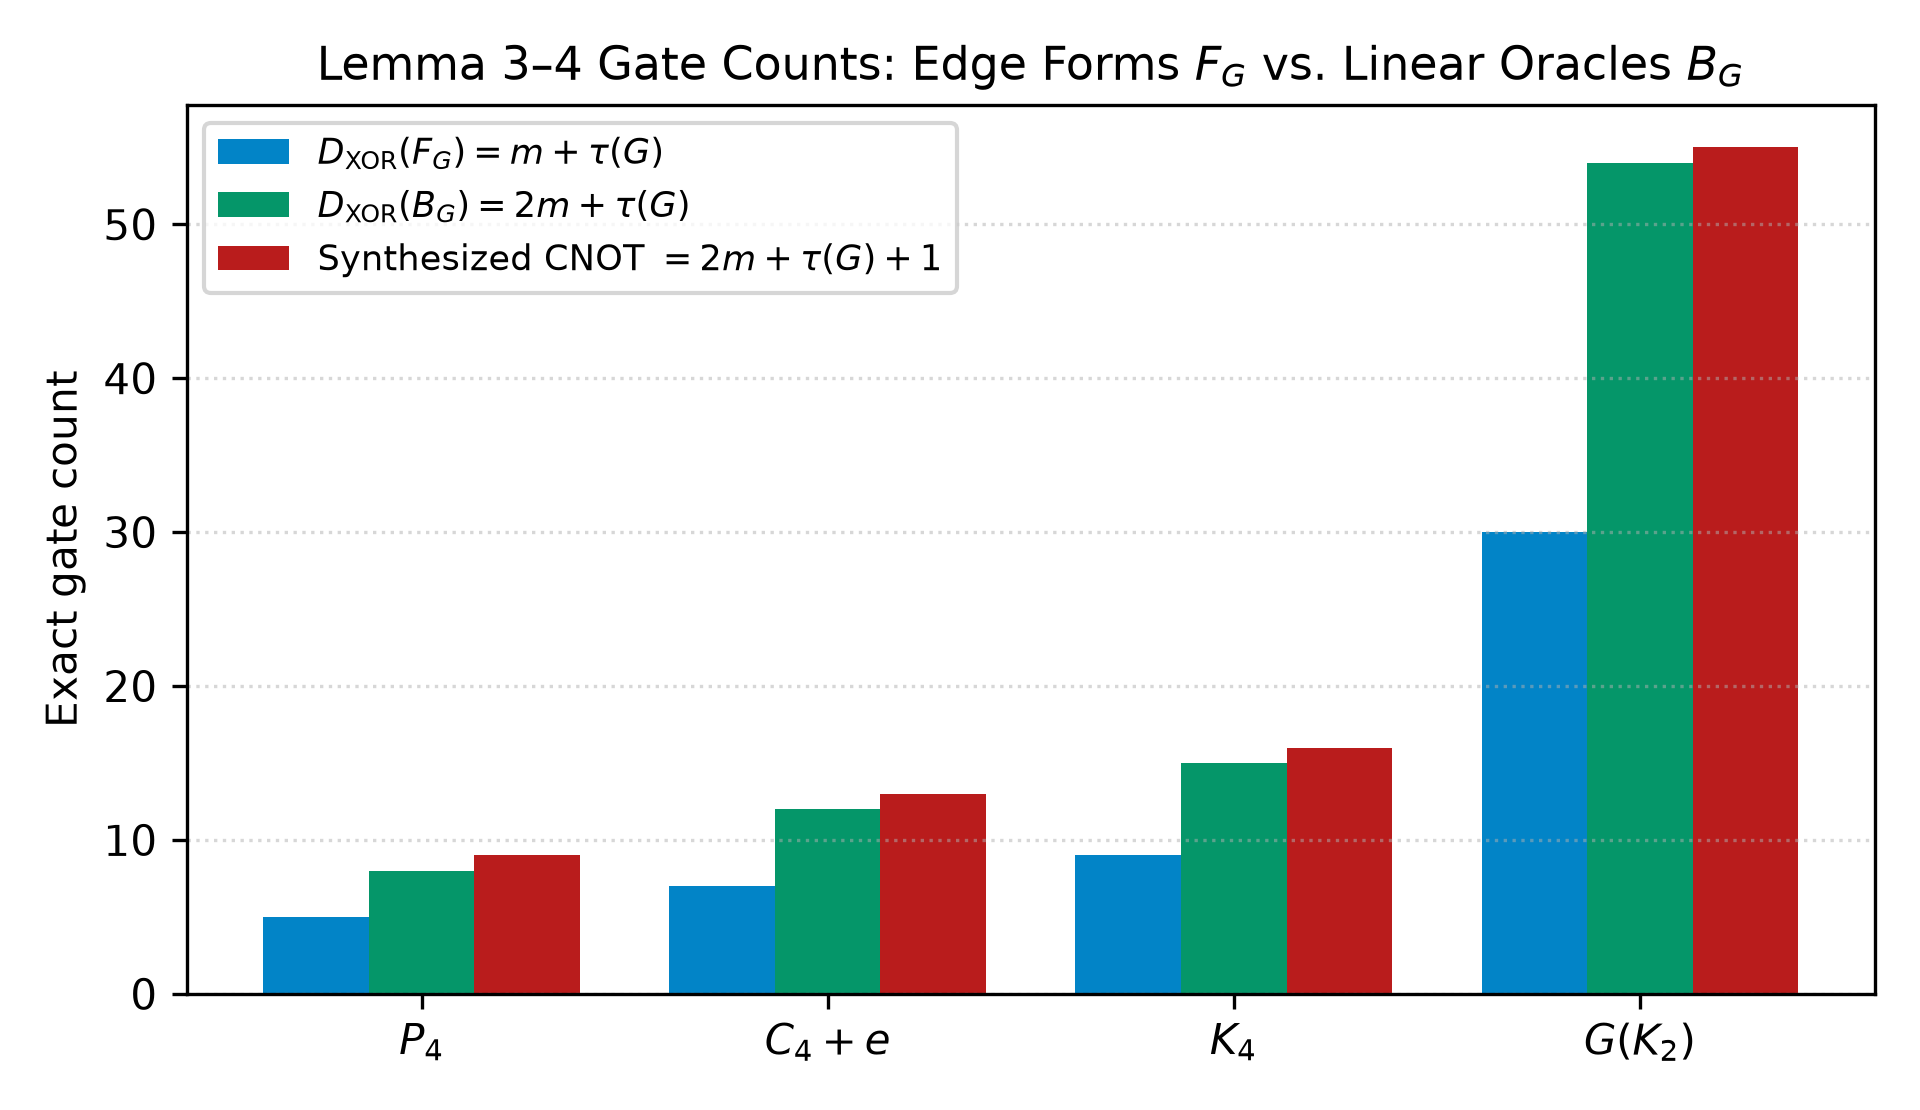
\includegraphics[width=\linewidth]{figures/fig1_xor_cnot_oracle_counts.png}
  \caption{Exact XOR distance $D_{\mathrm{XOR}}(F_G) = m+\tau(G)$, reversible XOR distance $D_{\mathrm{XOR}}(B_G) = 2m+\tau(G)$, and synthesized Lemma~4 CNOT gate count $2m+\tau(G)+1$ across \texttt{C09}--\texttt{C12}.}
  \label{fig:l4}
\end{figure}

\paragraph{Mode 4 (\texttt{free\_resources\_and\_parity\_thm5}, \texttt{C13}--\texttt{C16}).}
Verifies Theorem~5's even-$\tau$ parity-rounding decision equivalence ($\tau(G) \le k \iff D_{\mathrm{CNOT}}(B_G) \le 2m + k' + 1$, Fig.~\ref{fig:thm5}) on YES and NO instances, and executes Pavlogiannis's syntactic translation from CNOT circuits augmented with free SWAP gates and clean ancillas (0-control no-op, 0-target copy, SWAP wire relabeling) to an XOR circuit of at most $\#\text{CNOT}$ gates, confirming exact wire-by-wire output agreement over $\mathbb{F}_2$ and compliance with the $2m+\tau(G)$ lower bound.

\begin{figure}[t]
  \centering
  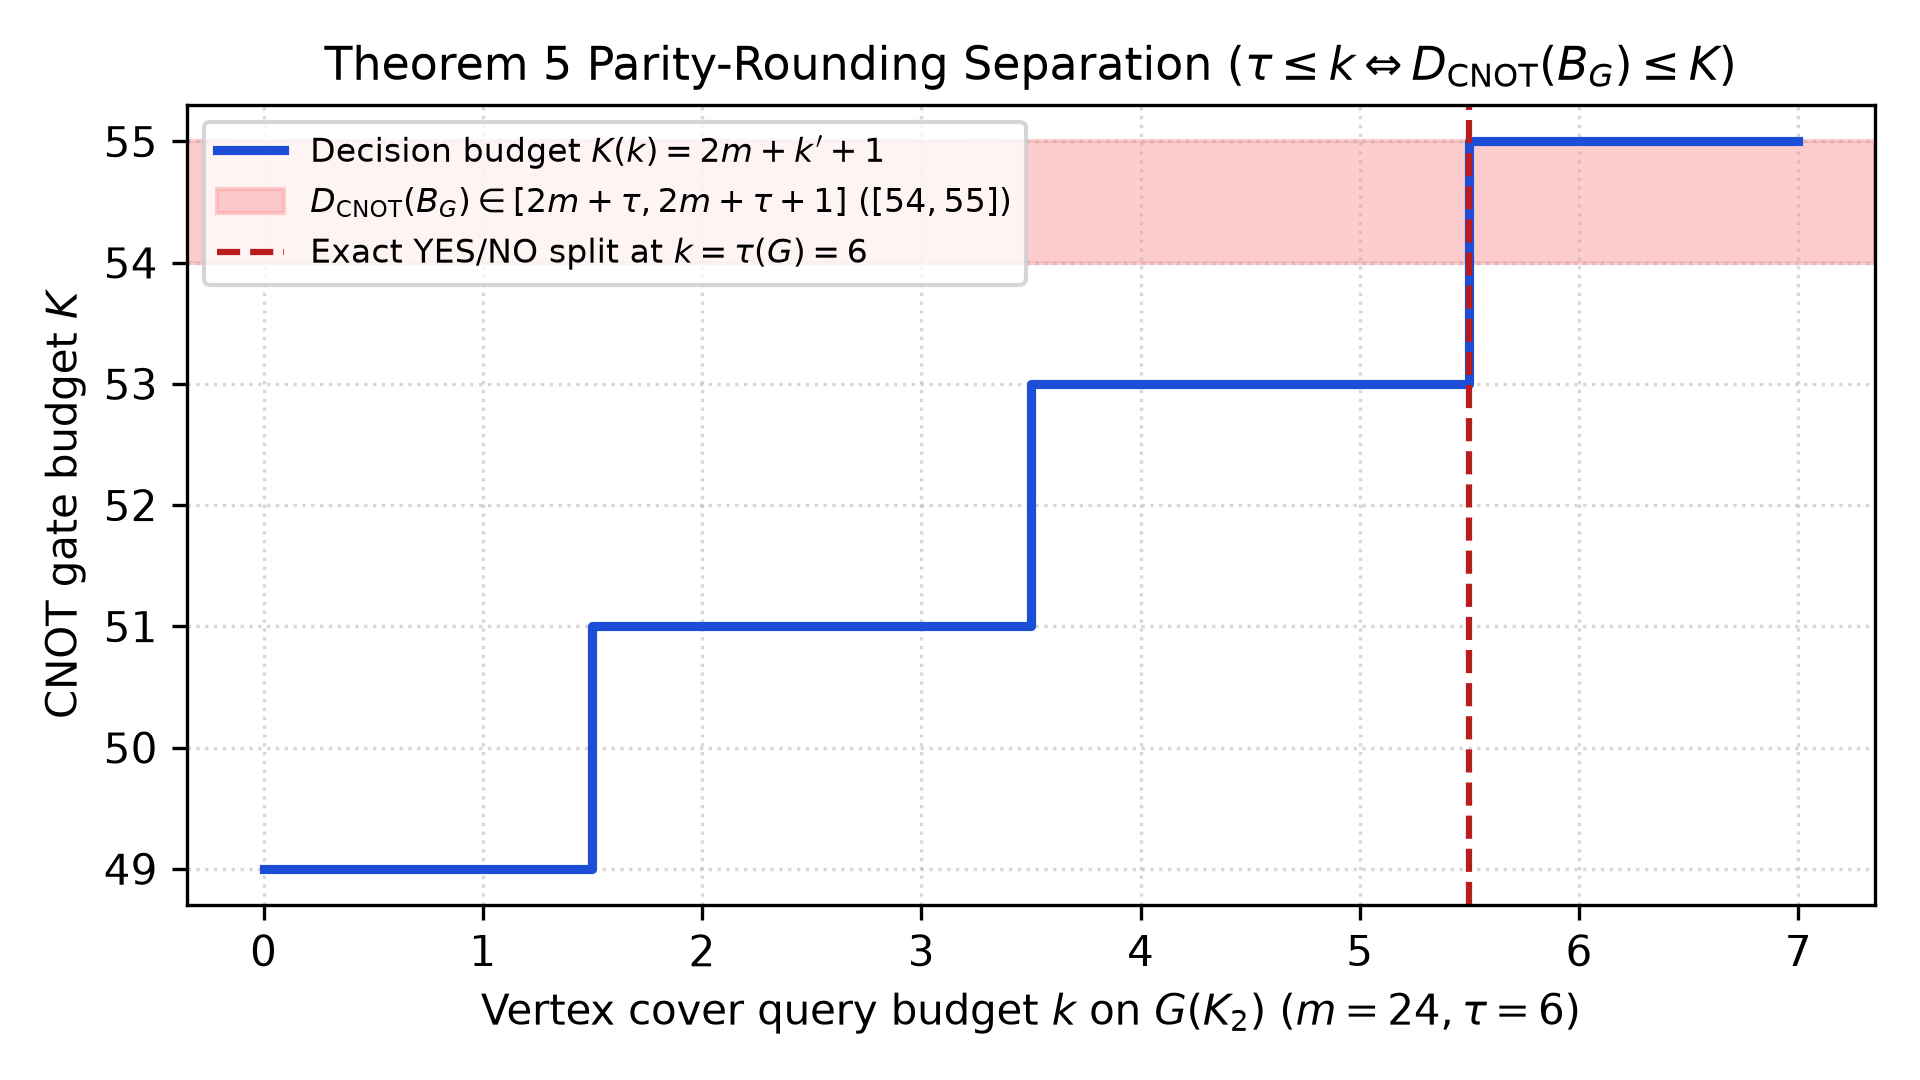
\includegraphics[width=\linewidth]{figures/fig3_theorem5_parity_gap.png}
  \caption{Theorem~5 parity-rounding decision budget $K(k) = 2m + k' + 1$ on $G(K_2)$ ($m=24, \tau=6$), cleanly separating YES ($k \ge 6$) and NO ($k \le 5$) instances around the Lemma~4 band $[54, 55]$.}
  \label{fig:thm5}
\end{figure}

\section{Certificate Suite and Adversarial Testing}

Table~\ref{tab:certs} summarizes all 16 canonical certificates (\texttt{C01}--\texttt{C16}). Our test suite (\path{tests/test_verifier.py}) executes 36 tests in under $0.25\text{ s}$: all 16 certificates, the AST zero-float audit, a \texttt{C13} zero-control/zero-target reduction test (11 CNOTs translating to 9 XOR gates $\le K=9$), and 18 adversarial forgery-rejection tests covering schema/mode tampering, \texttt{bool}/float coercion, forged $\tau(H)/\tau(G)/D_{\mathrm{XOR}}/\text{CNOT}$ counts, incomplete or out-of-range XOR circuits, non-Hamiltonian and non-covering vertex sets in Mode~3, empty/incomplete circuits, odd-$\tau$ rejection, and flipped decisions in Mode~4, unknown gate ops, self-loops, and duplicate edges.

\begin{table}[t]
\centering
\caption{Certificate inventory (\texttt{CNOT-HARD-CERT-1.0}, 16/16 verified).}
\label{tab:certs}
\scriptsize
\setlength{\tabcolsep}{2.5pt}
\begin{tabular}{@{}llll@{}}
\toprule
ID & M & Graph / Instance & Exact Certified Witness \\
\midrule
C01 & 1 & $H=P_3 \to G(12)$ & $\tau(H)=1, \tau(G)=8$ even, Ham path \\
C02 & 1 & $H=K_3 \to G(12)$ & $\tau(H)=2, \tau(G)=10$ even, Ham path \\
C03 & 1 & $H=C_4 \to G(16)$ & $\tau(H)=2, \tau(G)=12$ (exact B\&B) \\
C04 & 1 & $H=K_{1,3} \to G(16)$ & $\tau(H)=1, \tau(G)=10$ (exact B\&B) \\
C05 & 2 & $P_4$, 5-gate XOR & Optimal Case (a) elimination, $D=5$ \\
C06 & 2 & $P_4$, 6-gate XOR & Case (b) merge elimination, $D=5$ \\
C07 & 2 & $C_5$, 8-gate XOR & Full telescoping elimination, $D=8$ \\
C08 & 2 & $K_4$, 9-gate XOR & Full telescoping elimination, $D=9$ \\
C09 & 3 & $P_4$, $\mathrm{GL}(8,2)$ & $B_G^2=I$, exact 9-gate CNOT sim. \\
C10 & 3 & $C_4+e$, $\mathrm{GL}(10,2)$ & $B_G^2=I$, exact 13-gate CNOT sim. \\
C11 & 3 & $K_4$, $\mathrm{GL}(11,2)$ & $B_G^2=I$, exact 16-gate CNOT sim. \\
C12 & 3 & $G(K_2)$, $\mathrm{GL}(33,2)$ & $B_G^2=I$, exact 55-gate CNOT sim. \\
C13 & 4 & $P_4$, $k=2$, anc+SWAP & YES ($K=9$), XOR trans.\ exact \\
C14 & 4 & $P_4$, $k=1 \to k'=0$ & NO ($K=7 < 8$), parity rounded \\
C15 & 4 & $C_4+e$, $k=3$, SWAP & YES ($K=13$), XOR trans.\ exact \\
C16 & 4 & $G(K_2)$, $k=5 \to k'=4$ & NO ($K=53 < 54$), full pipeline \\
\bottomrule
\end{tabular}
\end{table}

\section{Reproducibility and Disclosure}

All files are SHA-256 hashed in \texttt{MANIFEST.sha256} and archived at \url{https://github.com/lluiseriksson/optimal-cnot-hardness-certificates} (\texttt{v1.0.0}). Independent reproduction requires only Lean~4.35.0 and Python~3.10+:
\begin{quote}\raggedright\footnotesize\ttfamily
cd lean \&\& lake build \&\& cd ..\\
python scripts/generate\_certificates.py\\
python -m src.cnot\_hardness\_verifier certificates/\\
pytest -q
\end{quote}
\noindent\textbf{AI-Assisted Formalization Disclosure.} This verification artifact was authored by Lluis Eriksson using Google Antigravity for Lean~4 proof engineering, zero-float $\mathbb{F}_2$ Python verification scripting, test design, and manuscript preparation. Every verified claim is scoped strictly to the 18 Lean~4.35.0 theorems and 16 exact $\mathbb{F}_2$ certificates (\texttt{C01}--\texttt{C16}).

\begin{thebibliography}{2}
\bibitem{pavlogiannis2026cnot}
A.~Pavlogiannis,
\emph{On the Hardness of Optimal CNOT Circuits},
arXiv:2611.34138v1, November 2026.
\bibitem{boyar2013}
J.~Boyar, P.~Matthews, and R.~Peralta,
\emph{Logic Minimization Techniques with Applications to Cryptology},
Journal of Cryptology \textbf{26} (2013), 280--312.
\end{thebibliography}

\end{document}
